\documentclass[border=3pt]{standalone}

\usepackage{tikz}
\usepackage[latin1]{inputenc}
\usetikzlibrary{positioning, arrows.meta, decorations.markings,calc}
\renewcommand{\familydefault}{\sfdefault}

\begin{document}
		
	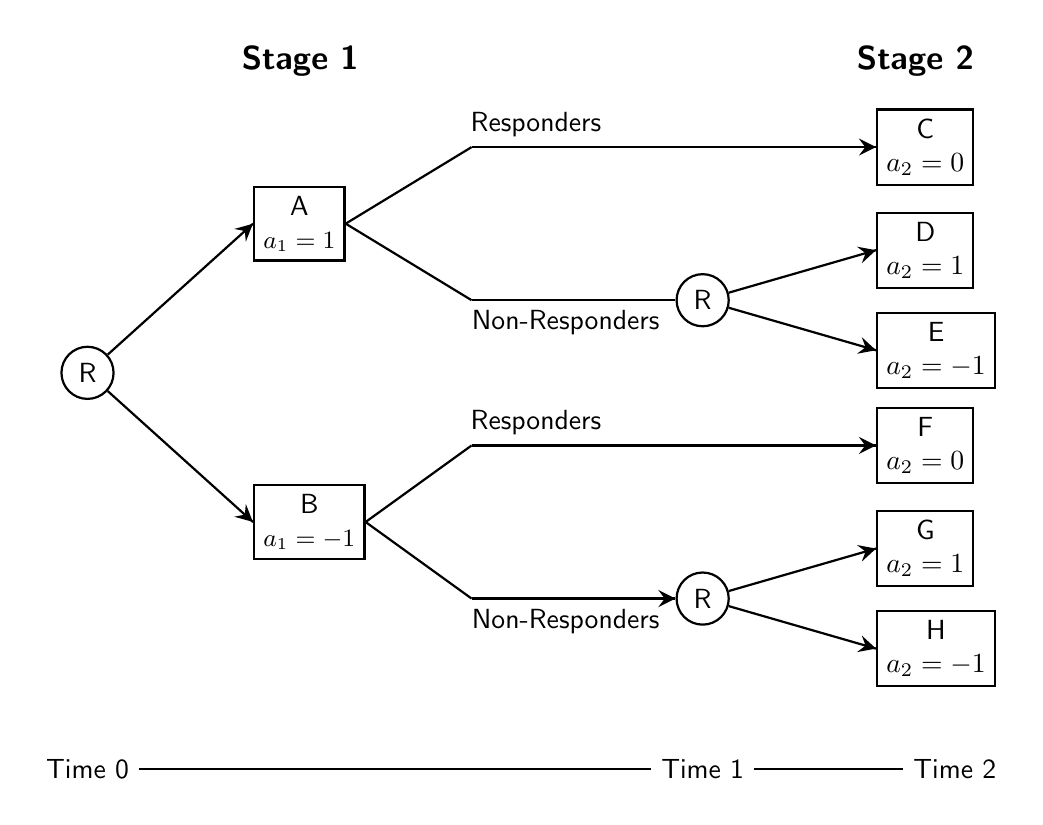
\begin{tikzpicture}[%
		node distance=6mm,
		randomize/.style={
			circle,
			minimum size=6mm,
			thick,
			black,
			draw
		},
		rerand/.style={
			xshift = 15mm
		},
		treatment/.style={
			rectangle,
			minimum size = 7mm,
			thick,
			black,
			anchor=west,
			align=center,
			draw
		},
		blank/.style={
			rectangle,
			minimum size=2mm
		},
		subgroup/.style={
			rectangle,
			rounded corners=1.5mm,
			thin,
			minimum size=6mm,
			black,
			draw
		},
		rlabel/.style={
%			font=\footnotesize,
			above,
			xshift=1mm,
			align=center
		},
		nrlabel/.style={
%			font=\footnotesize,
			below,
			xshift=-1mm,
			align=left
		},
		trialarrow/.style={
			thick,
			decoration={markings,mark=at position 1 with  {\arrow[scale=1.5,>=stealth]{>}}},
			postaction={decorate}
		},
		subsetarrow/.style={
			thin,
			decoration={markings,mark=at position 1 with {\arrow[scale=1.2,>=stealth]{>}}},
			postaction={decorate}
		}, thick]
						
		\matrix[row sep=-2mm,column sep=12mm] { %
			& \node [align=center,xshift=6mm] (stage1) {\large \textbf{Stage 1}}; & & & \node [align=center,xshift=5mm] (stage2) {\large \textbf{Stage 2}};\\[5mm]
			%
			%
			% DESIGN II
			
			\node (designII) [blank] {}; 
			& & \node (b1-II) [blank] {}; & \node (b2-II) [blank] {}; & \node (C-II) [treatment] {C \\ $a_{2} = 0$};\\
			& \node (stage1align) [treatment,white] {}; & & & \\
			& & & & \node (D-II) [treatment] {D \\ $a_{2} = 1$};\\
			& & \node (b3-II) [blank] {}; & \node (R2-II) [randomize, rerand] {R}; & \\
			& & & & \node (E-II) [treatment] {E \\ $a_{2} = -1$};\\			\node [randomize,white] {};  & & & & \\
			& & \node (b4-II) [blank] {}; & \node (b5-II) [blank] {}; & \node (F-II) [treatment] {F \\ $a_{2} = 0$};\\
			& \node [treatment, white] {}; & & & \\
			& & & & \node (G-II) [treatment] {G \\ $a_{2} = 1$};\\
			& & \node (b6-II) [blank] {}; & \node (R3-II) [randomize, rerand] {R}; & \\
			& & & & \node (H-II) [treatment] {H \\ $a_{2} = -1$};\\[1cm]
			
			% TIMEPOINTS
			
			\node (time0) [align=center, anchor=center] {Time 0};& & & \node (time1) [align=center, anchor=center, xshift=15mm] {Time 1}; & \node (time2) [align=center, xshift = 10mm] {Time 2}; \\
		};
	
%		\draw[dashed,lightgray] (time1.north) -- (R2-III.south);
%		\draw[dashed,lightgray] (R2-III.north) -- (R3-II.south);
%		\draw[dashed,lightgray] (R3-II.north) --++(90:3.2cm);
%		
%		\draw[dashed,lightgray] (time2.north west) --++(90:33cm);
	
		% DESIGN II LINES
		
		\draw let \p1 = (stage1align.west), \p2=($(C-II) !.5! (R2-II)$) in node[treatment] at (\x1, \y2) (A-II) {A \\ \small{$a_{1} = 1$}};
		
		\draw let \p1 = (stage1align.west), \p2=($(F-II) !.5! (R3-II)$) in node[treatment] at (\x1, \y2) (B-II) {B \\ \small{$a_{1} = -1$}};
		
		\draw let \p1 = (designII.north), \p2=($(A-II.north) !.5! (B-II.south)$) in node[randomize] at (\x1, \y2) (R1-II) {R};
		
%		\draw let \p3 = (stage1.north) \p4=($(C-II.north) !.5! (E-II.south)$) in node[treatment] at (\x3, \y4) (test) {A};
		
		
		
		\draw[trialarrow] (R1-II) -- (A-II.west);
		\draw (A-II.east) -- (b1-II.center);
		\draw (A-II.east) -- (b3-II.center);
		\draw (b1-II.center) -- node [rlabel] {Responders} (b2-II.center);
		\draw (b3-II.center) -- node [nrlabel] {Non-Responders} (R2-II);
		\draw[trialarrow] (b2-II.center) -- (C-II);
		\draw[trialarrow] (R2-II) -- (D-II.west);
		\draw[trialarrow] (R2-II) -- (E-II.west);
		
		\draw[trialarrow] (R1-II) -- (B-II.west);
		\draw (B-II.east) -- (b4-II.center);
		\draw (B-II.east) -- (b6-II.center);
		\draw (b4-II.center) -- node [rlabel] {Responders} (b5-II.center);
		\draw[trialarrow] (b5-II.center) -- (F-II);
		\draw[trialarrow] (b6-II.center) -- node [nrlabel] {Non-Responders} (R3-II);
		\draw[trialarrow] (R3-II) -- (G-II.west);
		\draw[trialarrow] (R3-II) -- (H-II.west);		
			
		% TIME LINES
		
		\draw (time0) -- (time1) -- (time2);
\end{tikzpicture}
\end{document}